\documentclass[degree=master, degreetype=profession, bibtype=numeric, newstyle=true]{tongjithesis}
% 选项:
%   degree=[master|doctor],                             % 必选, 硕士 | 博士
%   degreetype=[academic|profession|equaleducation],    % 可选, 学术型 | 专业型 | 同等学力, 默认为学术型
%   bibtype=[numeric|authoryear],                       % 可选, 数字式引用 | 作者-年份引用, 默认为数字式引用
%   newstyle,                                           % 可选, 是否使用新页眉格式 (居中格式), 默认已打开
%   pifootnote,                                         % 可选, 脚注是否用 ① 这种格式, 默认已打开
% 	electronic,                                         % 可选, 电子版标注: " 打印时删除 ", 默认已关闭
%   secret,                                             % 可选, 是否保密: 秘密 / 机密 / 绝密, 默认已关闭
%   encoding,                                           % 可选, 自定义西文编码 (默认无需定义, 详情请参考 fontenc 宏包文档)
%   注:默认已打开的选项可以使用 arialtitle=false 的形式关闭

% 其他文本格式 / 章节标题格式等选项可以参见 tongjithesis.cfg 中的说明, 按需要修改

% 兼容性提示: 旧版本的  wyqymathversion,   wyqyinputfile 仍然可用
%            分别等价于 tongjimathversion, tongjiinputfile


%%%%%%%%%%%%%%%%%%%%% 导言区 %%%%%%%%%%%%%%%%%%%%%
% 环境准备
\tongjimathversion{99}                                  % 填写本文件中 tongjiinputfile 命令的使用次数; 可以比实际数量多, 但不可少
\usepackage{tongjiutils}                                % 自定义宏放在这里, 包括一些常用指令
\addbibresource{ref/refs.bib}                           % 加入bib文件

%%%%%%%%%%%%%%%%%%%%% 正文区 %%%%%%%%%%%%%%%%%%%%%
\begin{document}

% 定义图片文件存放位置( 默认在 figures 子目录下 )
% 最好使用 pdf 格式的图片
\graphicspath{{figures/}}

%%% 封面部分
\frontmatter
\tongjiinputfile{data/cover} \makecover                 % 封面示例, 位置: data/cover.tex
\tableofcontents                                        % 目录( 自动生成 )
\tongjiinputfile[denotation]{data/denotation}             % 符号对照表示例, 位置: data/denotation.tex
%%% 以下索引按需要选择, 不需要的注释掉即可
\listoffigures                                          % 插图索引
\listoftables                                           % 表格索引
\listofalgorithms                                       % 算法索引
\listofequations                                        % 公式索引

%%% 正文部分
\mainmatter
% 用如下格式的命令插入文件, 格式: \tongjiinputfile[环境(可选参数)]{文件的相对路径}
\tongjiinputfile{data/chap01}                           % 第一章示例, 位置: data/chap01.tex
\tongjiinputfile{data/chap02}                           % 第二章示例, 位置: data/chap02.tex
\tongjiinputfile{data/chap03}                           % 第三章示例, 位置: data/chap03.tex
\tongjiinputfile{data/chap04}                           % 第四章示例, 位置: data/chap04.tex
\tongjiinputfile{data/chap05}                           % 第五章示例, 位置: data/chap05.tex

%%% 封底部分
\backmatter
\tongjiinputfile[acknowledgement]{data/ack}             % 致谢示例, 位置: data/ack.tex
\tongjiinputfile[reference]{ref/style}                  % 参考文献示例, 位置: data/ref.tex  
\tongjiinputfile[appendix]{data/appendix}               % 附录示例, 位置: data/appendix.tex
\tongjiinputfile[resume]{data/resume}                   % 个人简历示例, 位置: data/resume.tex
\tongjiinputfile[statements]{data/statements}           % 原创性声明和授权书( 仅供测试, 最终提交时请替换为自己的扫描件 )
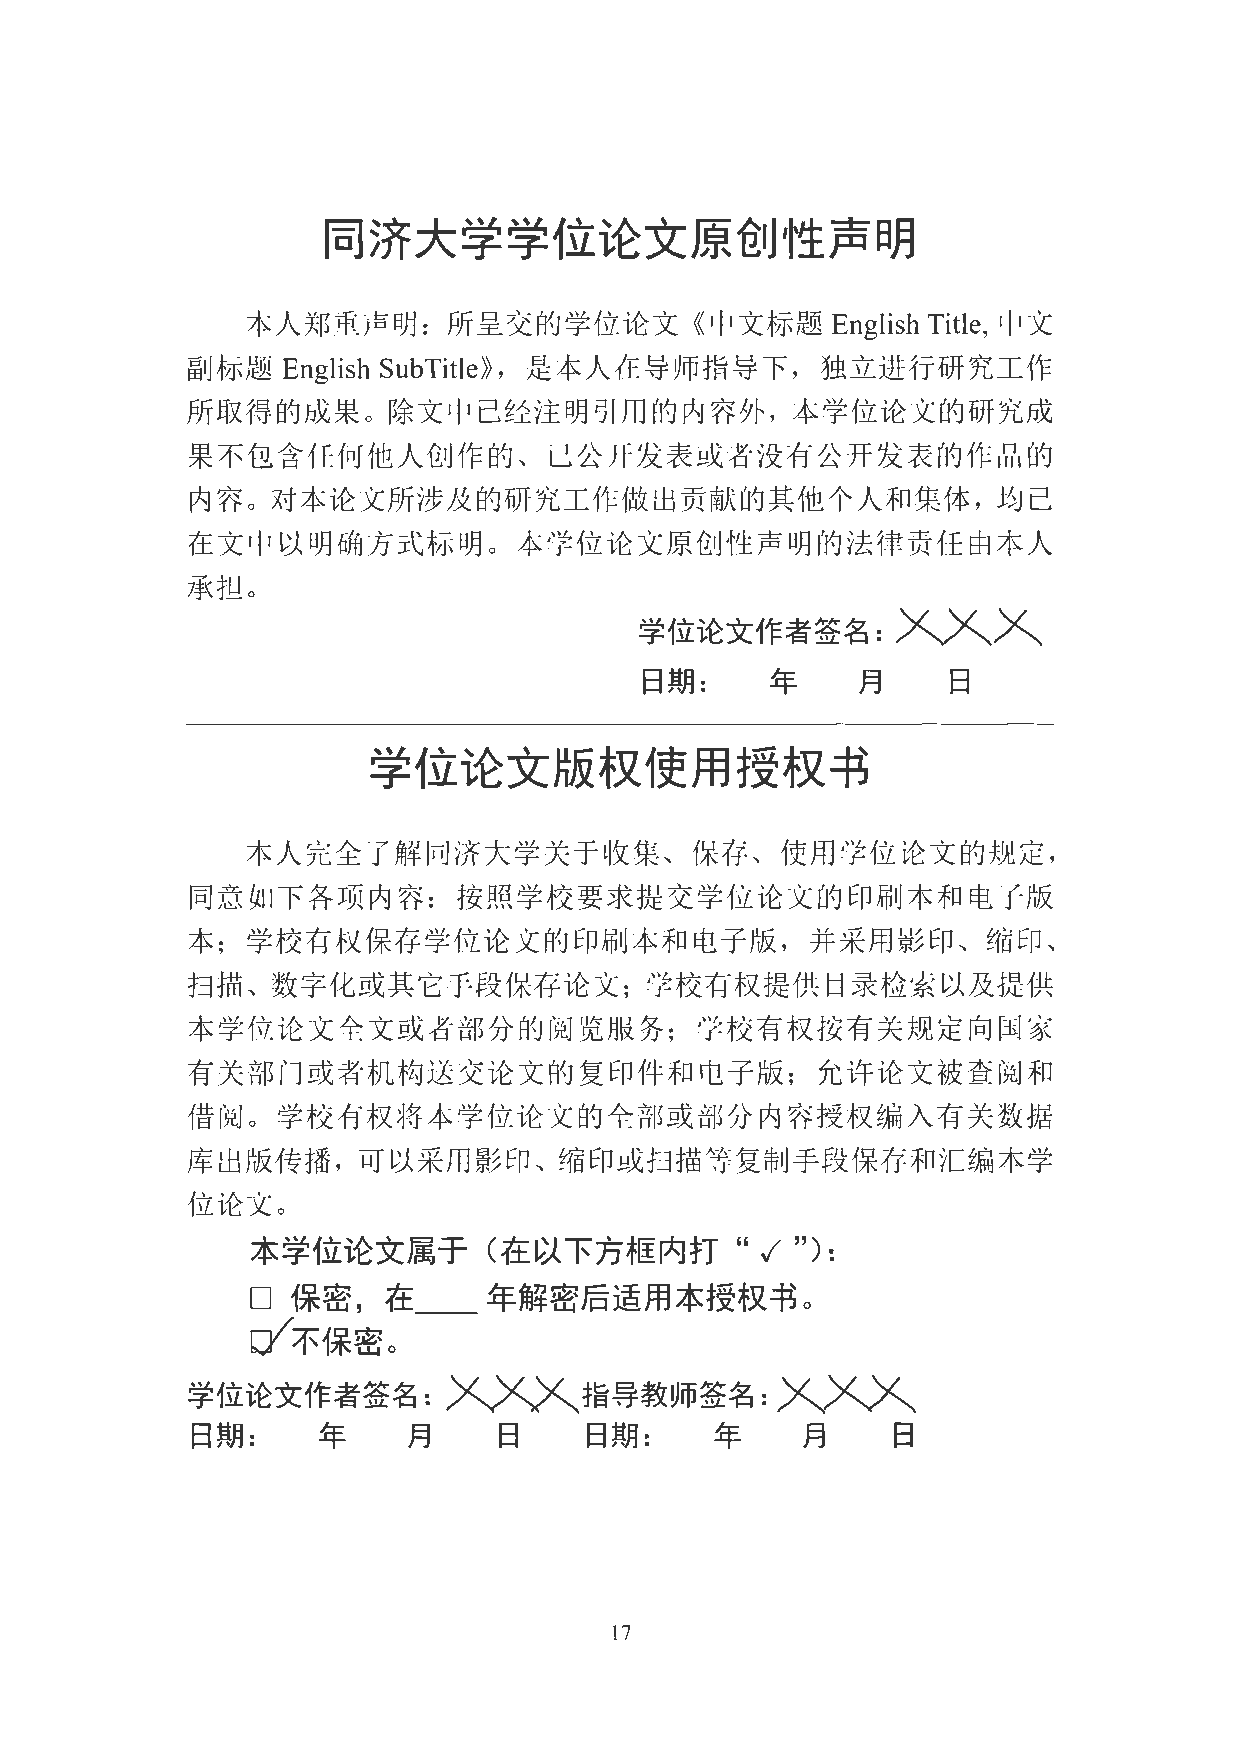
\includepdf{data/statements-scan.pdf}                   % 原创性声明和授权书扫描件( 仅供测试, 最终提交时请替换为自己的扫描件 )

\end{document}
